\chapter{Validation}
\label{chap:validation}

\vspace{-\baselineskip}

%##################################################################################################
\section{Chapter Overview}
%##################################################################################################

In order to evaluate the effectiveness of my approach, I undertook two separate pieces of validation work. The first piece involved quantifying the accuracy of the 3D feature identifiers presented in the previous chapter -- this was done by comparing their output to `gold standard' results produced manually in collaboration with a radiologist. The second piece involved validating the accuracy of my volume calculations (see \S\ref{sec:appendixapps-volumecalc}). To do this, I first manually identified the liver, kidneys and spleen in a number of series and used my program to calculate their volumes in each case. The volume results were then correlated with known weights provided by the radiologist (bearing in mind that the densities of the organs in question are relatively uniform).

Both producing the gold standard results and making inter-result comparisons involved implementing special features for the purpose in \emph{millipede}. For the gold standard production, manual drawing tools were implemented to allow the user to draw round features of interest in the images. The actual drawing was done using a \emph{Bamboo Fun} pen tablet manufactured by Wacom (see Figure~\ref{fig:validation-pentablet-usage}), as this provides more accurate user control here than would a standard mouse. The inter-result comparisons were implemented as a dialog box allowing the user to compare multi-feature selections on a per-feature basis. The implementation of all the validation-specific features is discussed in Appendix~\ref{chap:appendixval}.

The validation work undertaken here forms an important part of the basis for the following chapter, in which I critically assess all the contributions claimed in the introduction.

%---
\stufigex{height=20cm}{validation/validation-pentablet-usage.png}{A typical user drawing round the right kidney using a `lasso' drawing tool similar to that found in common image-editing programs}{fig:validation-pentablet-usage}{p}
%---

%##################################################################################################
\section{Validation of 3D Feature Identifiers}
%##################################################################################################

\index{validation!of 3D feature identifiers|(}

To validate my 3D feature identifiers, I undertook four detailed case studies to test how well they worked on sets of slices from different series. An alternative approach of testing them on a larger number of series, but with less detailed individual analysis, would also have been possible, but in my view further work must be done on improving the robustness of the identifiers before such larger-scale validation really makes sense. Furthermore, such larger-scale validation is a sizeable project in and of itself, and arguably beyond the scope of doctoral work. The aim here is mainly to illustrate some of the areas in which the identifiers currently succeed or fail in order to highlight areas for further work.

For each case study, I produced a `gold standard' result by manually identifying the aorta, kidneys, liver, ribs, spinal canal, spine and spleen using the validation tools described in Appendix~\ref{chap:appendixval}. The resulting features were checked, and corrected where necessary, by Dr Zoe Traill, a Consultant Radiologist at the Churchill Hospital, Oxford. I then identified the same features using the automated multi-feature identifier. To perform a comparison, the gold standard result ($G$) and automated result ($A$) were used to construct three derivative multi-feature selections:
%
\begin{enumerate}
\item $A - G$, which contains the parts of the features that were identified by the automated identifier but should not have been.
\item $G - A$, which contains the parts of the features that were missed by the automated identifier.
\item $A \cap G$, which contains the parts of the features that were correctly identified.
\end{enumerate}
%
These were then used to calculate the Dice similarity coefficient for each feature, as described in \S\ref{sec:appendixval-featurecomparisons}, providing a quantitative measure of the extent to which the automated and gold standard results correspond. Dice similarity coefficients range from $0$ to $1$, with $1$ indicating a perfect correspondence between two results and $0$ indicating that they do not correspond at all.

%################################################
\subsection{Series BT-2, Slices $60$--$80$}
%################################################

The first case study is of slices $60$--$80$ from series $2$ of a patient known as BT. Side-by-side comparisons of the automated and gold standard results are shown in Table~\ref{tbl:validation-BT-2-60-80} and Figure~\ref{fig:validation-BT-2-60-80}. The identified features can be analysed as follows:
%
\begin{itemize}

\item \textbf{Aorta}. As quantified by the relatively high Dice similarity coefficient of $0.859$ in Table~\ref{tbl:validation-BT-2-60-80}, the automated result for the aorta corresponds fairly well to the gold standard in this case. However, as shown in Figure~\ref{fig:validation-BT-2-60-80}(c), the automated result does flood slightly beyond the aorta itself. Referring back to one of the original slices (see Figure~\ref{fig:validation-BT-2-60-80-aorta-weakedge}), this is because the boundary between the aorta and an adjacent blood vessel (the left renal vein) is quite weak, and the stratified region growing algorithm thus does not know when to stop. This could perhaps be rectified by using level sets instead of region growing. A further problem is that the automated result slightly undersegments the outer boundary, as shown in Figure~\ref{fig:validation-BT-2-60-80}(d). This is primarily an issue with the original segmentation produced when constructing the partition forest.

\item \textbf{Kidneys}. Only the right kidney was relevant in this case, as the left kidney had been entirely overtaken by a huge tumour. As indicated by the high Dice similarity coefficient of $0.949$, the automated result for the kidney that was present was good. The minor discrepancies are primarily due to the automated identifier slightly oversegmenting the region around the renal pelvis.

\item \textbf{Liver}. Given the relative complexity of liver identification compared to identifying other features, the automated result in this case is fairly good, with a Dice similarity coefficient of $0.890$. However, Figure~\ref{fig:validation-BT-2-60-80}(d) illustrates that the lateral segment of the left lobe is clearly missed. This is due to the current approach doing only single-seed region growing -- in the slices chosen, the lateral segment of the left lobe and the rest of the liver are not connected (see Figure~\ref{fig:validation-BT-2-60-80-liver-disconnected}), so the algorithm finds one part of the liver but not the other. This could be rectified in this case by using multi-seed region growing, although some care would need to be taken over choosing appropriate seeds to make sure that other features in the area were not mistakenly identified as being part of the liver. A further problem with the automated liver result is that it floods beyond the boundary of the liver in the direction of the aorta (see Figure~\ref{fig:validation-BT-2-60-80}(c)). As with the aorta result, this is due to a weak boundary, and a level sets approach might be more effective.

\item \textbf{Ribs}. The ribs are identified reasonably well in this case, with a Dice similarity coefficient of $0.773$. The main source of inaccuracy, as can be seen in Figures~\ref{fig:validation-BT-2-60-80}(c) and (d), is that the automated identifier has incorrectly identified the top-most ribs as spine (hence Table~\ref{tbl:validation-BT-2-60-80} contains a high $G - A$ value for ribs). As was mentioned in the previous chapter, this is a known problem with the current ribs identifier, in that it deliberately avoids marking as rib anything that has already been marked as spine, thus giving priority to the spine where there is a conflict between the two. This is considered a suitable area for further work.

\item \textbf{Spinal Canal}. The spinal canal identifier works fairly well here, with a Dice similarity coefficient of $0.840$. The number of missed voxels ($309$) is relatively small in comparison to the overall size of the canal; the more significant issue is that the spinal canal has been somewhat oversegmented, hence the slightly high value for $A - G$ in this case. The major reason for this is that the spinal canal identifier currently works by filtering for suitable branch nodes (see Listing~\ref{code:featureid-3d-spinalcanalidentification}), and this relies on regions in the partition forest being exactly the right shape. For the spinal canal, this is roughly the case, which is why the approach works reasonably well. However, waterfall hierarchies converge relatively quickly (i.e.~the number of nodes in each layer decreases rapidly as we go towards the top of the forest) -- by the time enough smaller regions inside the spinal column have been merged to form a suitable region that can be identified as the spinal canal, surrounding regions inside the spinal column have usually been dragged in as well, ultimately leading to oversegmentation of the spinal canal (see Figure~\ref{fig:validation-BT-2-60-80-spinalcanal-oversegmentation}). A possible way of improving the situation would be to use the outer contour of the existing result (which is generally fairly good) to initialise a level set method that could be used to refine the boundary.

\item \textbf{Spine}. As witnessed by a high Dice similarity coefficient of $0.926$, the spine identifier produces relatively good results in this case. However, as mentioned earlier, there is a tendency for the spine to be oversegmented at the expense of the ribs when there is a conflict between them. Furthermore, as can be seen in Figure~\ref{fig:validation-BT-2-60-80}(d), the automated identifier often misses the \emph{transverse processes} of the spine (that is, the pieces that protrude to the left and right of the main spinal column). This is primarily because it currently uses a branch node filtering approach (see Listing~\ref{code:featureid-3d-spineidentification}), and the processes are not generally merged into the main spine region during forest construction (see Figure~\ref{fig:validation-BT-2-60-80-spine-transverseprocesses}). Since the primary aim of the spine identifier in this thesis is to provide a landmark that can be used when identifying other organs, this is not considered to be a major issue for our purposes here, but further work could be done to improve the identifier in this regard.

\item \textbf{Spleen}. Despite the relatively incipient nature of the spleen identifier, it performs in some ways surprisingly well on the BT-2 case study, with a Dice similarity coefficient of $0.853$. At present, however, the identifier undersegments the spleen because it accepts the initial spleen seed as is, without attempting to grow a full spleen feature from it (see Listing~\ref{code:featureid-3d-spleenidentification}). Ultimately, it may be sensible to use the spleen seed to initialise a level sets approach, but this is a subject for further work.

\end{itemize}

%---
\begin{table}[p]
\begin{center}
\begin{tabular}{c|cccccc}
\footnotesize \textbf{Feature} & \footnotesize \textbf{Automated (A)} & \footnotesize \textbf{Gold (G)} & \footnotesize \textbf{A -- G} & \footnotesize \textbf{G -- A} & \footnotesize \textbf{A $\cap$ G} & \footnotesize \textbf{Dice} \\
\hline
\footnotesize Aorta & \footnotesize 13940 & \footnotesize 13973 & \footnotesize 1949 & \footnotesize 1982 & \footnotesize 11991 & \footnotesize 0.859 \\
\footnotesize Kidneys & \footnotesize 72142 & \footnotesize 73715 & \footnotesize 2915 & \footnotesize 4488 & \footnotesize 69227 & \footnotesize 0.949 \\
\footnotesize Liver & \footnotesize 180156 & \footnotesize 180693 & \footnotesize 19624 & \footnotesize 20161 & \footnotesize 160532 & \footnotesize 0.890 \\
\footnotesize Ribs & \footnotesize 22787 & \footnotesize 31125 & \footnotesize 1942 & \footnotesize 10280 & \footnotesize 20845 & \footnotesize 0.773 \\
\footnotesize Spinal Canal & \footnotesize 14451 & \footnotesize 11002 & \footnotesize 3758 & \footnotesize 309 & \footnotesize 10693 & \footnotesize 0.840 \\
\footnotesize Spine & \footnotesize 111889 & \footnotesize 113385 & \footnotesize 7634 & \footnotesize 9130 & \footnotesize 104255 & \footnotesize 0.926 \\
\footnotesize Spleen & \footnotesize 11841 & \footnotesize 15077 & \footnotesize 359 & \footnotesize 3595 & \footnotesize 11482 & \footnotesize 0.853 \\
\end{tabular}
\end{center}
\caption{A numeric comparison of the automated and gold standard results for the BT-2-60-80 feature identification case study. (All entries except those for the similarity coefficient are in voxels.)}
\label{tbl:validation-BT-2-60-80}
\end{table}
%---

%---
\begin{stusubfig}{p}
	\subfigure[Automated Result ($A$)]
	{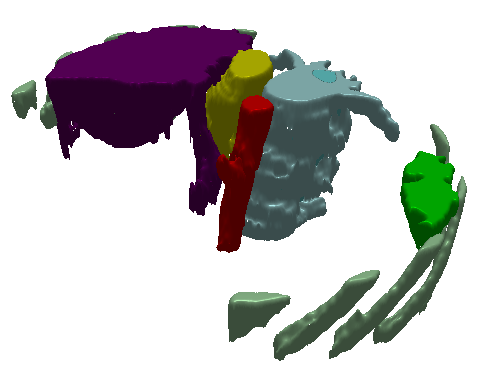
\includegraphics[width=.45\linewidth]{validation/validation-BT-2-60-80-target.png}}%
	%
	\hspace{4mm}%
	%
	\subfigure[Gold Standard Result ($G$)]
	{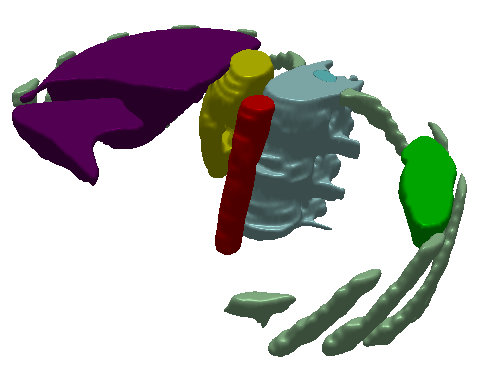
\includegraphics[width=.45\linewidth]{validation/validation-BT-2-60-80-goldstandard.png}}%
	%
	\\
	%
	\subfigure[$A - G$]
	{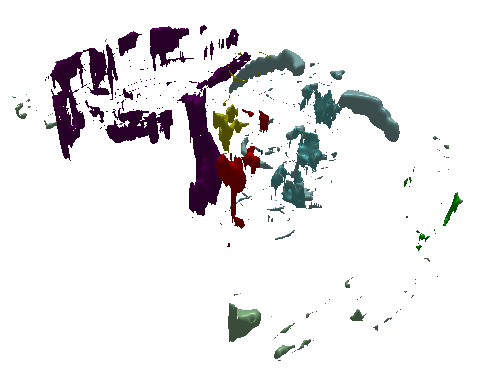
\includegraphics[width=.45\linewidth]{validation/validation-BT-2-60-80-TminusG.png}}%
	%
	\hspace{4mm}%
	%
	\subfigure[$G - A$]
	{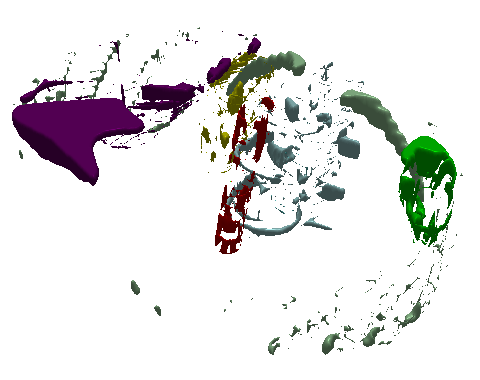
\includegraphics[width=.45\linewidth]{validation/validation-BT-2-60-80-GminusT.png}}%
\caption{A visual comparison of the automated and gold standard results for the BT-2-60-80 feature identification case study}
\label{fig:validation-BT-2-60-80}
\end{stusubfig}
%---

%---
\stufigex{height=8cm}{validation/validation-BT-2-60-80-aorta-weakedge-labelled.png}{The aorta identifier can flood into adjacent blood vessels, such as the left renal vein, due to weak boundaries in the original images}{fig:validation-BT-2-60-80-aorta-weakedge}{p}
%---

%---
\stufigex{height=8cm}{validation/validation-BT-2-60-80-liver-disconnected-labelled.png}{The liver identifier misses the lateral segment of the left lobe in the BT-2 case study because it is not connected to the rest of the liver in the slices chosen}{fig:validation-BT-2-60-80-liver-disconnected}{p}
%---

%---
\stufigex{height=8cm}{validation/validation-BT-2-60-80-spinalcanal-oversegmentation.png}{The spinal canal tends to be slightly oversegmented, with surrounding voxels, such as those marked in blue, identified when they should not be}{fig:validation-BT-2-60-80-spinalcanal-oversegmentation}{p}
%---

%---
\begin{stusubfig}{p}
	\subfigure[]
	{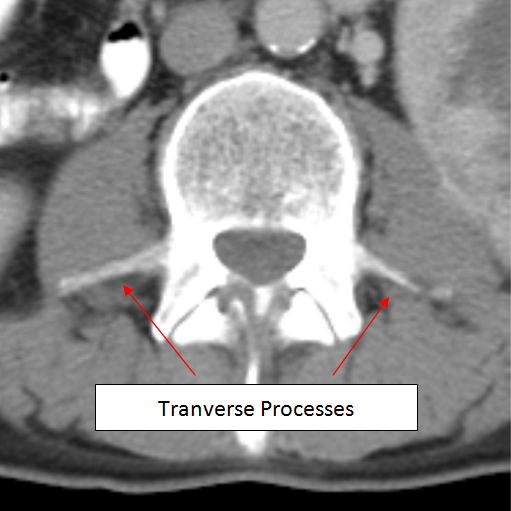
\includegraphics[width=.45\linewidth]{validation/validation-BT-2-60-80-spine-transverseprocesses-a-labelled.png}}%
	%
	\hspace{4mm}%
	%
	\subfigure[]
	{
\includegraphics[width=.45\linewidth]{validation/validation-BT-2-60-80-spine-transverseprocesses-b.png}}%
\caption{The spine identifier misses the transverse processes of the spine (a) in the BT-2 case study, because the hierarchical segmentation process does not merge them into the main spine region (b)}
\label{fig:validation-BT-2-60-80-spine-transverseprocesses}
\end{stusubfig}
%---

\afterpage{\clearpage}
\newpage

%################################################
\subsection{Series SD-2, Slices $70$--$90$}
%################################################

The second case study is of slices $70$--$90$ from series $2$ of a patient known as SD. Side-by-side comparisons of the automated and gold standard results are shown in Table~\ref{tbl:validation-SD-2-70-90} and Figure~\ref{fig:validation-SD-2-70-90}. The identified features can be analysed as follows:
%
\begin{itemize}

\item \emph{Aorta}. As with the BT-2 series, the aorta is identified fairly well in this case (with a Dice similarity coefficient of $0.811$), but there is the same tendency as there to flood into neighbouring blood vessels somewhat. Figure~\ref{fig:validation-SD-2-70-90}(c) illustrates that the liver has also flooded out too far in this series, which interferes with the bottom part of the aorta in the figures (although note that since multi-feature selections can overlap, this only affects the visualization of the aorta and not its underlying identification result).

\item \emph{Kidneys}. Only the left kidney was relevant in this case, as the patient had previously undergone a nephrectomy on their right kidney (i.e.~their right kidney had been taken out). The automated result for the left kidney is good (with a Dice similarity coefficient of $0.931$), although it is not quite as smooth as the gold standard in places. This is primarily an issue with the underlying hierarchical segmentation (see Figure~\ref{fig:validation-SD-2-70-90-kidneys-difference}).

\item \emph{Liver}. The automated liver result is good in this case (with a Dice similarity coefficient of $0.932$). Unlike in the BT-2 case study, no major part of the liver is missed here, because the liver is connected in the slices chosen. However, as before, there is flooding beyond the boundary of the liver in the direction of the aorta, due to weak edges in the image.

\item \emph{Ribs}. Whilst the ribs result is fairly good overall, with a Dice similarity coefficient of $0.819$, there are nevertheless some problems to be tackled. One of these is that the automated identifier can sometimes erroneously identify small, bright regions in the image that look like ribs but are actually unrelated (see Figure~\ref{fig:validation-SD-2-70-90-ribs-extraneous}). Whilst an attempt has been made to exclude such regions based on size or location in the image (see Listing~\ref{code:featureid-3d-ribsidentification}), better localization will ultimately be necessary to eliminate this problem. A further issue is that small parts of several ribs are missed because they appear greyer than usual in the images -- as shown in Figure~\ref{fig:validation-SD-2-70-90}(d), which shows the parts of features that have been missed, this is a relatively minor problem as far as each individual rib is concerned, but it is somewhat more significant from a statistical standpoint.

\item \emph{Spinal Canal}. The spinal canal has been relatively well identified in this case, with a Dice similarity coefficient of $0.862$ and only $101$ voxels missed. However, as in the BT-2 case study (and for the same reasons), it is oversegmented within the spinal column.

\item \emph{Spine}. The spine is particularly well identified in this case (with a Dice similarity coefficient of $0.965$). This is primarily a result of this patient's notably high bone density (notice how white the spine appears in Figure~\ref{fig:validation-SD-2-70-90-ribs-extraneous}(a)). There are some minor boundary differences between the automated identification and gold standard, but these do not greatly affect the results.

\item \emph{Spleen}. As in the BT-2 case, the spleen identifier performs relatively well given that it is currently at an early stage of development -- the result here has a Dice similarity coefficient of $0.874$. Whilst the automated result currently misses some of the spleen and contains a number of holes, a major part of the spleen has been successfully identified, providing at least a sensible basis for further work.

\end{itemize}

%---
\begin{table}[p]
\begin{center}
\begin{tabular}{c|cccccc}
\footnotesize \textbf{Feature} & \footnotesize \textbf{Automated (A)} & \footnotesize \textbf{Gold (G)} & \footnotesize \textbf{A -- G} & \footnotesize \textbf{G -- A} & \footnotesize \textbf{A $\cap$ G} & \footnotesize \textbf{Dice} \\
\hline
\footnotesize Aorta & \footnotesize 12799 & \footnotesize 9848 & \footnotesize 3619 & \footnotesize 668 & \footnotesize 9180 & \footnotesize 0.811 \\
\footnotesize Kidneys & \footnotesize 93853 & \footnotesize 91324 & \footnotesize 7671 & \footnotesize 5142 & \footnotesize 86182 & \footnotesize 0.931 \\
\footnotesize Liver & \footnotesize 254945 & \footnotesize 231766 & \footnotesize 28156 & \footnotesize 4977 & \footnotesize 226789 & \footnotesize 0.932 \\
\footnotesize Ribs & \footnotesize 10331 & \footnotesize 10097 & \footnotesize 1962 & \footnotesize 1728 & \footnotesize 8369 & \footnotesize 0.819 \\
\footnotesize Spinal Canal & \footnotesize 15163 & \footnotesize 11655 & \footnotesize 3609 & \footnotesize 101 & \footnotesize 11554 & \footnotesize 0.862 \\
\footnotesize Spine & \footnotesize 84757 & \footnotesize 85430 & \footnotesize 2624 & \footnotesize 3297 & \footnotesize 82133 & \footnotesize 0.965 \\
\footnotesize Spleen & \footnotesize 46129 & \footnotesize 55049 & \footnotesize 1922 & \footnotesize 10842 & \footnotesize 44207 & \footnotesize 0.874 \\
\end{tabular}
\end{center}
\caption{A numeric comparison of the automated and gold standard results for the SD-2-70-90 feature identification case study. (All entries except those for the similarity coefficient are in voxels.)}
\label{tbl:validation-SD-2-70-90}
\end{table}
%---

%---
\begin{stusubfig}{p}
	\subfigure[Automated Result ($A$)]
	{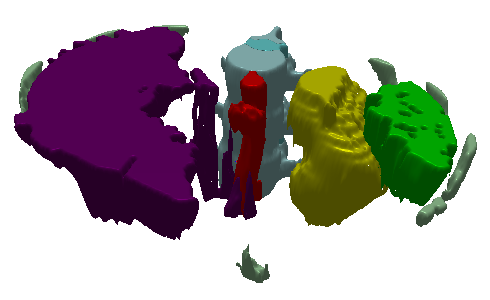
\includegraphics[width=.45\linewidth]{validation/validation-SD-2-70-90-target.png}}%
	%
	\hspace{4mm}%
	%
	\subfigure[Gold Standard Result ($G$)]
	{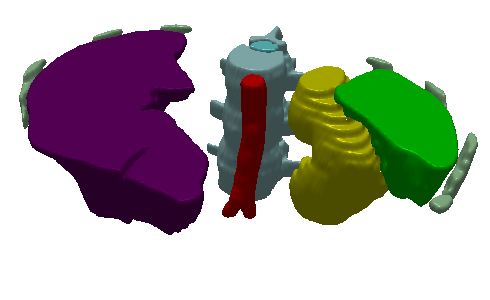
\includegraphics[width=.45\linewidth]{validation/validation-SD-2-70-90-goldstandard.png}}%
	%
	\\
	%
	\subfigure[$A - G$]
	{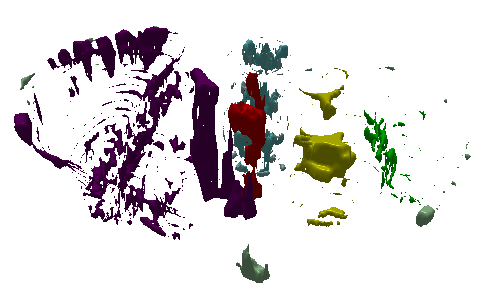
\includegraphics[width=.45\linewidth]{validation/validation-SD-2-70-90-TminusG.png}}%
	%
	\hspace{4mm}%
	%
	\subfigure[$G - A$]
	{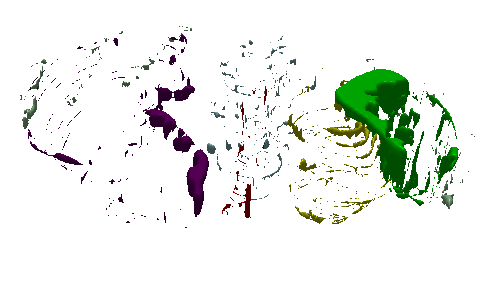
\includegraphics[width=.45\linewidth]{validation/validation-SD-2-70-90-GminusT.png}}%
\caption{A visual comparison of the automated and gold standard results for the SD-2-70-90 feature identification case study}
\label{fig:validation-SD-2-70-90}
\end{stusubfig}
%---

%---
\begin{stusubfig}{p}
	\subfigure[]
	{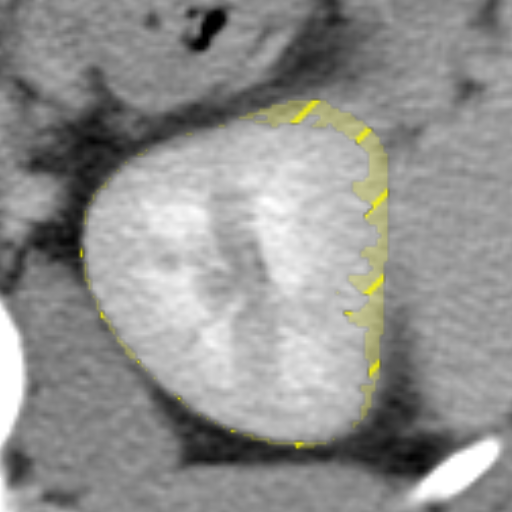
\includegraphics[width=.45\linewidth]{validation/validation-SD-2-70-90-kidneys-difference-a.png}}%
	%
	\hspace{4mm}%
	%
	\subfigure[]
	{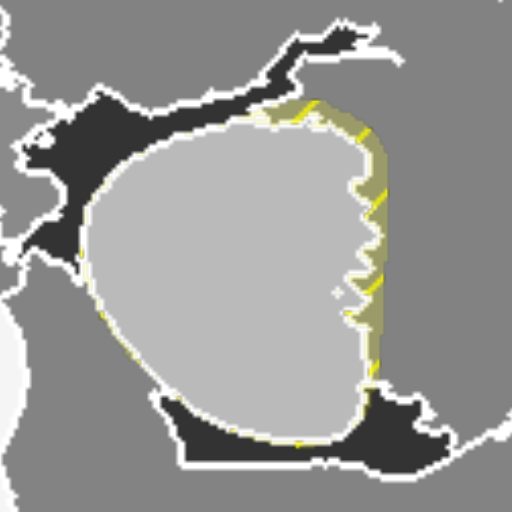
\includegraphics[width=.45\linewidth]{validation/validation-SD-2-70-90-kidneys-difference-b.png}}%
\caption{The difference (shown in yellow) between the gold standard and automated kidneys identification results for SD-2 is due to the underlying hierarchical segmentation, as seen in (b) -- the automated result identifies just the main kidney region, missing the real boundary in places}
\label{fig:validation-SD-2-70-90-kidneys-difference}
\end{stusubfig}
%---

%---
\begin{stusubfig}{p}
	\subfigure[]
	{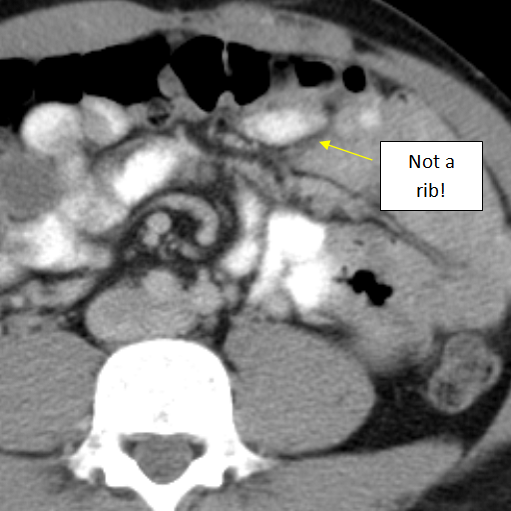
\includegraphics[width=.45\linewidth]{validation/validation-SD-2-70-90-ribs-extraneous-a-labelled.png}}%
	%
	\hspace{4mm}%
	%
	\subfigure[]
	{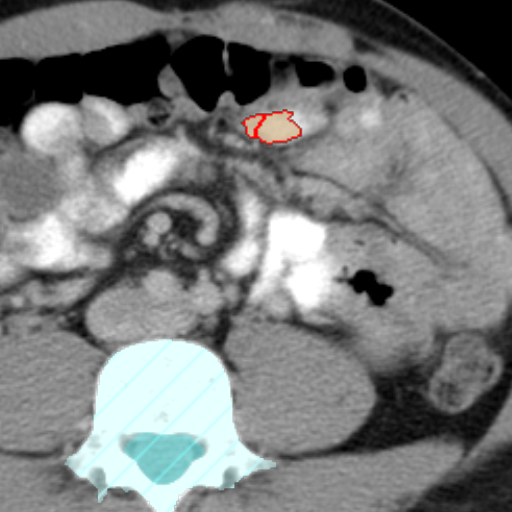
\includegraphics[width=.45\linewidth]{validation/validation-SD-2-70-90-ribs-extraneous-b.png}}%
\caption{The ribs identifier can sometimes erroneously identify small, bright regions of the image as ribs -- better localization is needed to prevent such mistakes}
\label{fig:validation-SD-2-70-90-ribs-extraneous}
\end{stusubfig}
%---

\afterpage{\clearpage}
\newpage

%################################################
\subsection{Series MC-2, Slices $110$--$130$}
%################################################

The third case study is of slices $110$--$130$ from series $2$ of a patient known as MC. Side-by-side comparisons of the automated and gold standard results are shown in Table~\ref{tbl:validation-MC-2-110-130} and Figures~\ref{fig:validation-MC-2-110-130} and \ref{fig:validation-MC-2-110-130-differences}. The identified features can be analysed as follows:
%
\begin{itemize}

\item \emph{Aorta}. As can be seen in Figures~\ref{fig:validation-MC-2-110-130}(c) and (d), the aorta is identified well in this case, with a Dice similarity coefficient of $0.908$. The differences there are largely due to the underlying hierarchical segmentation. A more noticeable issue in this case is that the automated liver result has flooded out too far (see Figure~\ref{fig:validation-MC-2-110-130})(a), obscuring the generally correct aorta result. A partial way of fixing this in the specific case shown here would be to unidentify as liver anything also marked as aorta, find the connected components of the remaining liver and keep only the largest one -- however, this would not solve the underlying problem of weak edges around the liver.

\item \emph{Kidneys}. The kidneys result for this case is quite good, with a Dice similarity coefficient of $0.906$. However, both kidneys suffer from oversegmentation, as can be seen in Figure~\ref{fig:validation-MC-2-110-130-differences}(c). In the case of the left kidney, this is caused by a weak edge (see Figure~\ref{fig:validation-MC-2-110-130-leftkidney-weakedge}). For the right kidney, it is due to a subjective difference in how the kidney ought to be segmented -- the automated result chooses to include the renal pelvis in the segmentation result (see Figure~\ref{fig:validation-MC-2-110-130-rightkidney-difference}(a)), whilst the gold standard chooses to exclude it (see Figure~\ref{fig:validation-MC-2-110-130-rightkidney-difference}(b)). Note that in both cases, the automated result is less `stair-stepped' than the gold standard -- this is not surprising, because the slices in the image volume used are quite thick ($5\mathit{mm}$) and the gold standard was produced by drawing round the kidneys slice-by-slice, which inevitably leads to a somewhat stair-stepped result.

\item \emph{Liver}. Although a reasonable overall shape is obtained for the liver, it is clear from the huge number of extraneous voxels ($108454$) that the automated identifier has failed in this case. The primary problem is that the stratified region growing process has flooded beyond the boundary of the liver and into surrounding features -- in this case, the liver's connecting blood vessels. Once in the vascular system, the flooding can keep going, even to the extent that it encompasses the aorta. As mentioned in \S\ref{subsec:featureid-3d-liveridentification}, one potential solution to this is to initially identify only the liver seed and then use that to initialise a level sets method that can constrain the curvature of the contour to try and avoid going too far beyond the boundary of the liver. This would be a suitable avenue for further work.

Another problem with the liver identification in this case is that it misses both the medial segment and part of the lateral segment of the liver's left lobe (see Figures~\ref{fig:validation-MC-2-110-130-liver-medialsegment} and \ref{fig:validation-MC-2-110-130-differences}(b)). The major reason for this is that the mean grey values of the liver regions in this case are all clustered around the lower threshold of $150$ used by the liver identifier for region growing (see Listing~\ref{code:featureid-3d-liveridentification}). The medial segment and the part of the lateral segment that is missed have mean grey values that are just below the threshold chosen. Whilst this could be rectified for this particular case by simply lowering the threshold, this is not an appropriate solution to the more general problem, which is that if thresholds are chosen, they need to depend on the properties of the individual images. Absolute thresholds do not work well in this case, because there is a great deal of variation between different CT series.

\item \emph{Ribs}. As witnessed by a Dice similarity coefficient of $0.816$, the ribs identifier produces a reasonably good result in this case. However, Figures~\ref{fig:validation-MC-2-110-130-differences}(c) and (d) reveal two key problems to be tackled. The first problem is that, as in the BT-2 case, the top-most ribs have been identified as spine instead of rib, leading to a high number ($11565$) of missed rib voxels overall. Further work is necessary to refine the precise boundaries between the two. The second problem is that the ribs generated by the automated identifier (see Figure~\ref{fig:validation-MC-2-110-130}(c)) contain holes in places. This is primarily due to parts of some of the ribs being greyer than usual in this series (see Figure~\ref{fig:validation-MC-2-110-130-ribs-toogrey}).

\newpage

\item \emph{Spinal Canal}. The spinal canal is identified well in this case, with a Dice similarity coefficient of $0.933$. As in previous cases, however, the automated result is slightly oversegmented, for the same reasons as outlined there.

\item \emph{Spine}. The spine result is good in this case, with a Dice similarity coefficient of $0.947$. The main issue to be tackled is that the top-most ribs are inadvertently identified as spine rather than rib here, as previously mentioned. As in the BT-2 case, the identifier also misses the transverse processes of the spine in places.

\item \emph{Spleen}. As in previous cases, the spleen identifier primarily suffers from undersegmentation here. It produces what is in many ways a promising result (with a Dice similarity coefficient of $0.898$), but is not yet at the point where it can fully identify the spleen as a whole.

\end{itemize}

%---
\begin{table}[p]
\begin{center}
\begin{tabular}{c|cccccc}
\footnotesize \textbf{Feature} & \footnotesize \textbf{Automated (A)} & \footnotesize \textbf{Gold (G)} & \footnotesize \textbf{A -- G} & \footnotesize \textbf{G -- A} & \footnotesize \textbf{A $\cap$ G} & \footnotesize \textbf{Dice} \\
\hline
\footnotesize Aorta & \footnotesize 15799 & \footnotesize 15036 & \footnotesize 1805 & \footnotesize 1042 & \footnotesize 13994 & \footnotesize 0.908 \\
\footnotesize Kidneys & \footnotesize 148065 & \footnotesize 137416 & \footnotesize 18698 & \footnotesize 8049 & \footnotesize 129367 & \footnotesize 0.906 \\
\footnotesize Liver & \footnotesize 492435 & \footnotesize 413475 & \footnotesize 108454 & \footnotesize 29494 & \footnotesize 383981 & \footnotesize 0.848 \\
\footnotesize Ribs & \footnotesize 33626 & \footnotesize 42708 & \footnotesize 2483 & \footnotesize 11565 & \footnotesize 31143 & \footnotesize 0.816 \\
\footnotesize Spinal Canal & \footnotesize 9924 & \footnotesize 9087 & \footnotesize 1054 & \footnotesize 217 & \footnotesize 8870 & \footnotesize 0.933 \\
\footnotesize Spine & \footnotesize 81483 & \footnotesize 79453 & \footnotesize 5247 & \footnotesize 3217 & \footnotesize 76236 & \footnotesize 0.947 \\
\footnotesize Spleen & \footnotesize 32048 & \footnotesize 36537 & \footnotesize 1240 & \footnotesize 5729 & \footnotesize 30808 & \footnotesize 0.898 \\
\end{tabular}
\end{center}
\caption{A numeric comparison of the automated and gold standard results for the MC-2-110-130 feature identification case study. (All entries except those for the similarity coefficient are in voxels.)}
\label{tbl:validation-MC-2-110-130}
\end{table}
%---

%---
\begin{stusubfig}{p}
	\subfigure[Automated Result ($A$)]
	{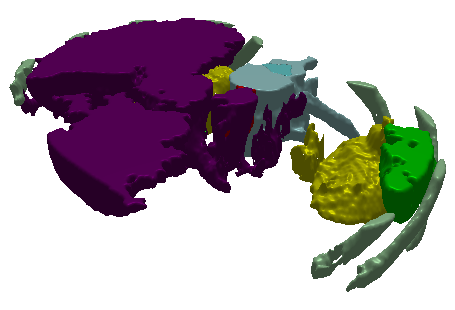
\includegraphics[width=.45\linewidth]{validation/validation-MC-2-110-130-target.png}}%
	%
	\hspace{4mm}%
	%
	\subfigure[Gold Standard Result ($G$)]
	{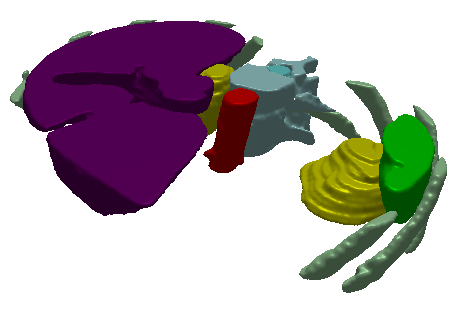
\includegraphics[width=.45\linewidth]{validation/validation-MC-2-110-130-goldstandard.png}}%
	%
	\\
	%
	\subfigure[Automated Result Excluding Liver ($A'$)]
	{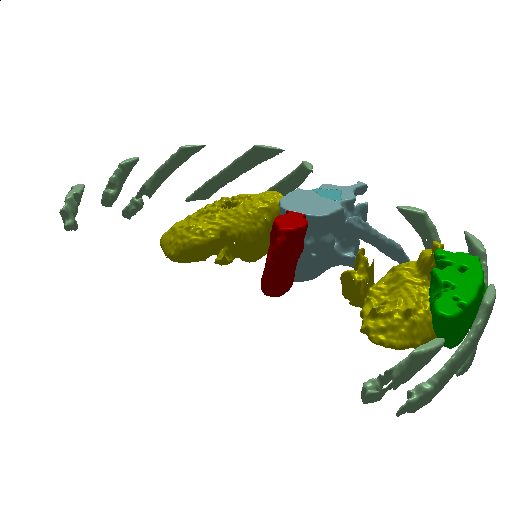
\includegraphics[width=.45\linewidth]{validation/validation-MC-2-110-130-target-noliver.png}}%
	%
	\hspace{4mm}%
	%
	\subfigure[Gold Standard Result Excluding Liver ($G'$)]
	{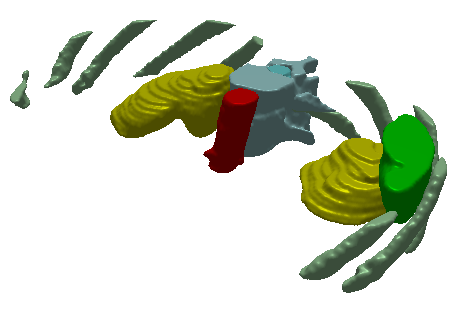
\includegraphics[width=.45\linewidth]{validation/validation-MC-2-110-130-goldstandard-noliver.png}}%
\caption{A visual comparison of the automated and gold standard results (with and without the liver) for the MC-2-110-130 feature identification case study}
\label{fig:validation-MC-2-110-130}
\end{stusubfig}
%---

%---
\begin{stusubfig}{p}
	\subfigure[$A - G$]{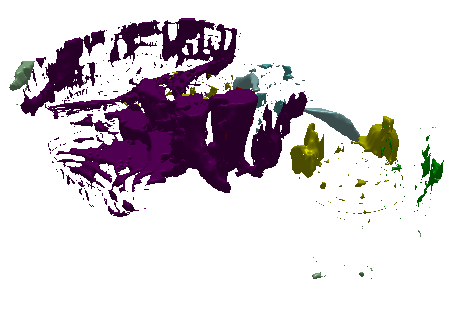
\includegraphics[width=.45\linewidth]{validation/validation-MC-2-110-130-TminusG.png}}%
	\hspace{4mm}%
	\subfigure[$G - A$]{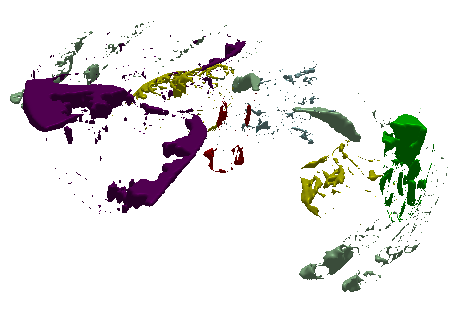
\includegraphics[width=.45\linewidth]{validation/validation-MC-2-110-130-GminusT.png}}%
	\\
	\subfigure[$A' - G'$]{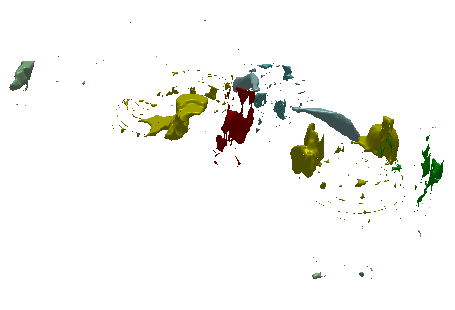
\includegraphics[width=.45\linewidth]{validation/validation-MC-2-110-130-TminusG-noliver.png}}%
	\hspace{4mm}%
	\subfigure[$G' - A'$]{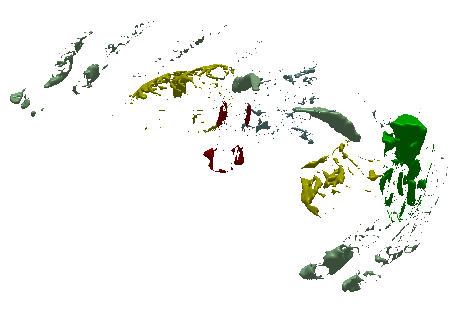
\includegraphics[width=.45\linewidth]{validation/validation-MC-2-110-130-GminusT-noliver.png}}%
\caption{The differences between the automated and gold standard results (with and without the liver) shown in Figure~\ref{fig:validation-MC-2-110-130}}
\label{fig:validation-MC-2-110-130-differences}
\end{stusubfig}
%---

%---
\begin{stusubfig}{p}
	\subfigure[]
	{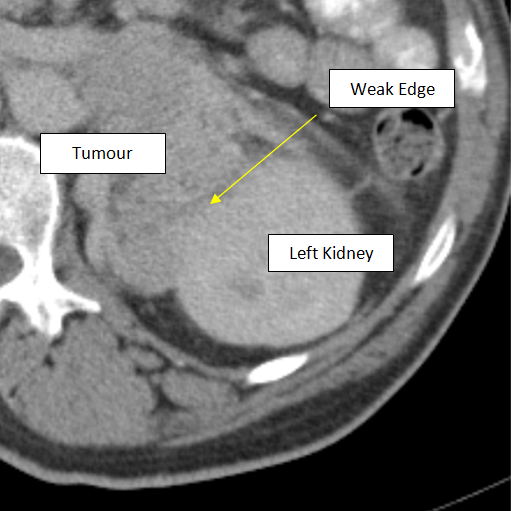
\includegraphics[width=.45\linewidth]{validation/validation-MC-2-110-130-leftkidney-weakedge-a-labelled.png}}%
	%
	\hspace{4mm}%
	%
	\subfigure[]
	{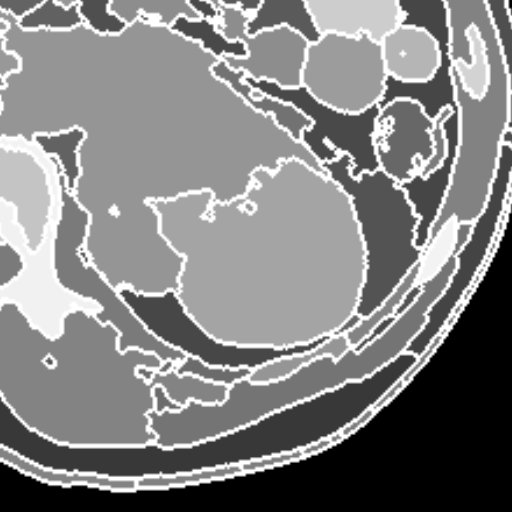
\includegraphics[width=.45\linewidth]{validation/validation-MC-2-110-130-leftkidney-weakedge-b.png}}%
\caption{MC's left kidney shares a weak edge with an adjoining tumour (a) -- this leads to a less than perfect segmentation of the image (b), and causes the automated identifier to oversegment the left kidney}
\label{fig:validation-MC-2-110-130-leftkidney-weakedge}
\end{stusubfig}
%---

%---
\begin{stusubfig}{p}
	\subfigure[Automated Result]
	{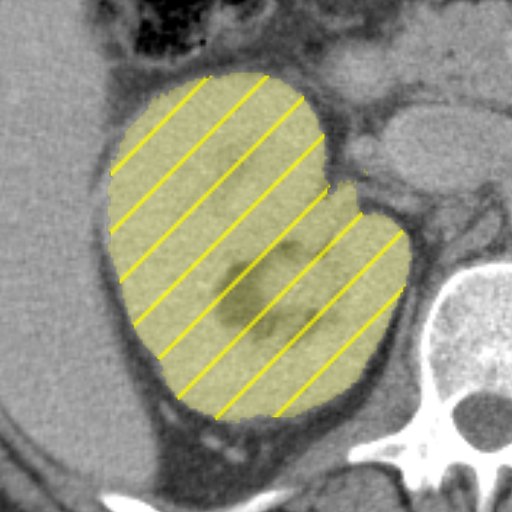
\includegraphics[width=.45\linewidth]{validation/validation-MC-2-110-130-rightkidney-difference-a.png}}%
	%
	\hspace{4mm}%
	%
	\subfigure[Gold Standard]
	{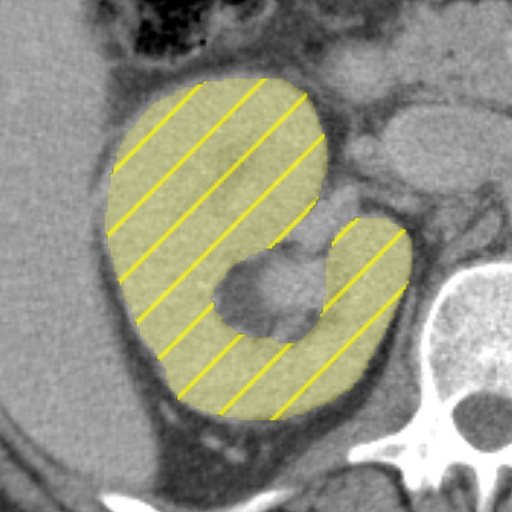
\includegraphics[width=.45\linewidth]{validation/validation-MC-2-110-130-rightkidney-difference-b.png}}%
\caption{The automated result for MC's right kidney chooses to include the renal pelvis, whilst the gold standard chooses not to include it}
\label{fig:validation-MC-2-110-130-rightkidney-difference}
\end{stusubfig}
%---

%---
\stufigex{height=8cm}{validation/validation-MC-2-110-130-liver-medialsegment-labelled.png}{The locations of the medial and lateral segments of the left lobe of the liver -- parts of these are missed by the liver identifier in the MC-2 case study, because the mean grey values of many of the regions representing them are below the required threshold}{fig:validation-MC-2-110-130-liver-medialsegment}{p}
%---

%---
\stufigex{height=8cm}{validation/validation-MC-2-110-130-ribs-toogrey-labelled.png}{Parts of MC's ribs appear greyer than usual on the CT scans, causing them to be missed by the ribs identifier}{fig:validation-MC-2-110-130-ribs-toogrey}{p}
%---

\afterpage{\clearpage}
\newpage

%################################################
\subsection{Series EB-2, Slices $60$--$80$}
%################################################

The final case study is of slices $60$--$80$ from series $2$ of a patient known as EB. Side-by-side comparisons of the automated and gold standard results are shown in Table~\ref{tbl:validation-EB-2-60-80} and Figure~\ref{fig:validation-EB-2-60-80}. The identified features can be analysed as follows:
%
\begin{itemize}

\item \emph{Aorta}. The aorta result is reasonable in this case, with a Dice similarity coefficient of $0.849$. However, there is some flooding into adjacent blood vessels at the top of the aorta due to weak image edges. Part of the aorta is also undersegmented at the bottom due to calcification of the artery, which manifests itself as bright regions in the CT scans.

\item \emph{Kidneys}. As can be seen in Figures~\ref{fig:validation-EB-2-60-80}(a) and (b), the right kidney result is good in this case (having a Dice similarity coefficient of $0.932$). Where there are minor differences, these are primarily around the renal pelvis. The left kidney, on the other hand, is completely missed by the automated identifier due to a large tumour (see Figure~\ref{fig:validation-EB-2-60-80-leftkidney-tumour}).

\item \emph{Liver}. The liver is identified well here, with a Dice similarity coefficient of $0.948$. However, some pieces of the liver are still missed, as shown in Figure~\ref{fig:validation-EB-2-60-80}(d). Specifically, the small piece of the lateral segment of the left lobe at the front of the liver is missed because it is disconnected from the rest of the liver in the slices chosen, and small parts of the right lobe and the medial segment of the left lobe are missed because the mean grey values of the regions representing them are slightly below the chosen threshold of $150$. Note that both of these issues were also observed in the previous case studies, suggesting that they are not series-specific. This will be discussed further when critically assessing the liver identifier in the next chapter.

\item \emph{Ribs}. The ribs result is poor in this case, with a Dice similarity coefficient of only $0.488$. The primary cause is oversegmentation, due to this series containing many small, bright regions in the image that are not ribs (much like the example shown in Figure~\ref{fig:validation-SD-2-70-90-ribs-extraneous} for the SD-2 case study). Whilst the current ribs identifier does manage to exclude some of these regions on size grounds, a better localization approach is needed to overcome this problem more generally.

\item \emph{Spinal Canal}. As witnessed by a Dice similarity coefficient of $0.856$, the spinal canal result is quite good in this case. However, as in previous cases, it is still somewhat oversegmented within the spinal column.

\item \emph{Spine}. The spine is identified fairly well in this case (with a Dice similarity coefficient of $0.925$), but as in previous cases, the transverse processes are missed. This is mainly because they tend to be darker than the rest of the spine on the scans, causing the grey level-based hierarchical segmentation approach used to merge them into surrounding regions rather than the spine. The automated identifier also slightly oversegments the spine in places (see Figure~\ref{fig:validation-EB-2-60-80}(c)), but in practice this amounts to relatively minor boundary issues spread over multiple slices (note that Figure~\ref{fig:validation-EB-2-60-80}(c) makes the result look worse than it is, because the oversegmentations of the spine and spinal canal appear in roughly the same place in the image).

\item \emph{Spleen}. As with the left kidney, the spleen is unfortunately completely missed in this case. This is because in the partition forest for this image volume, there is no suitable spleen seed in layer $1$ (see Figure~\ref{fig:validation-EB-2-60-80-spleen-missed}) due to the region merging performed by the waterfall being slower than usual here. The underlying cause of this is that the CT window (see \S\ref{subsubsec:segmentation-watershed-ct-windowing}) that the radiologists stored with the EB-2 images is $50/350$ rather than the usual $40/400$ abdominal window. This affects the brightness and contrast of the image, and hence the way in which regions are merged. (When a $40/400$ window is used, a slightly better spleen result is obtained.) A sensible way to handle this issue is to ensure that a consistent window is used when segmenting the images, and further work should take care to do this.

\end{itemize}

%---
\begin{table}[p]
\begin{center}
\begin{tabular}{c|cccccc}
\footnotesize \textbf{Feature} & \footnotesize \textbf{Automated (A)} & \footnotesize \textbf{Gold (G)} & \footnotesize \textbf{A -- G} & \footnotesize \textbf{G -- A} & \footnotesize \textbf{A $\cap$ G} & \footnotesize \textbf{Dice} \\
\hline
\footnotesize Aorta & \footnotesize 10365 & \footnotesize 9416 & \footnotesize 1969 & \footnotesize 1020 & \footnotesize 8396 & \footnotesize 0.849 \\
\footnotesize Kidney (Right) & \footnotesize 47444 & \footnotesize 46918 & \footnotesize 3461 & \footnotesize 2935 & \footnotesize 43983 & \footnotesize 0.932 \\
\footnotesize Kidney (Left) & \footnotesize 0 & \footnotesize 36874 & \footnotesize 0 & \footnotesize 36874 & \footnotesize 0 & \footnotesize 0.000 \\
\footnotesize Liver & \footnotesize 160978 & \footnotesize 164834 & \footnotesize 6592 & \footnotesize 10448 & \footnotesize 154386 & \footnotesize 0.948 \\
\footnotesize Ribs & \footnotesize 10256 & \footnotesize 4959 & \footnotesize 6542 & \footnotesize 1245 & \footnotesize 3714 & \footnotesize 0.488 \\
\footnotesize Spinal Canal & \footnotesize 12387 & \footnotesize 9645 & \footnotesize 2958 & \footnotesize 216 & \footnotesize 9429 & \footnotesize 0.856 \\
\footnotesize Spine & \footnotesize 82721 & \footnotesize 85490 & \footnotesize 4946 & \footnotesize 7715 & \footnotesize 77775 & \footnotesize 0.925 \\
\footnotesize Spleen & \footnotesize 0 & \footnotesize 20179 & \footnotesize 0 & \footnotesize 20179 & \footnotesize 0 & \footnotesize 0.000 \\
\end{tabular}
\end{center}
\caption{A numeric comparison of the automated and gold standard results for the EB-2-60-80 feature identification case study. (All entries except those for the similarity coefficient are in voxels.)}
\label{tbl:validation-EB-2-60-80}
\end{table}
%---

%---
\begin{stusubfig}{p}
	\subfigure[Automated Result ($A$)]
	{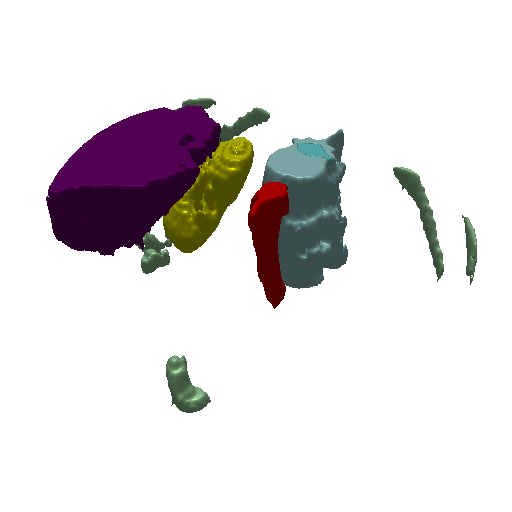
\includegraphics[width=.45\linewidth]{validation/validation-EB-2-60-80-target.png}}%
	%
	\hspace{4mm}%
	%
	\subfigure[Gold Standard Result ($G$)]
	{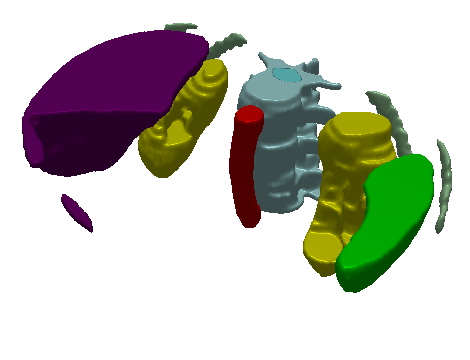
\includegraphics[width=.45\linewidth]{validation/validation-EB-2-60-80-goldstandard.png}}%
	%
	\\
	%
	\subfigure[$A - G$]
	{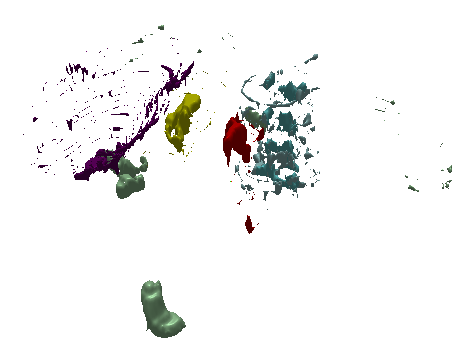
\includegraphics[width=.45\linewidth]{validation/validation-EB-2-60-80-TminusG.png}}%
	%
	\hspace{4mm}%
	%
	\subfigure[$G - A$]
	{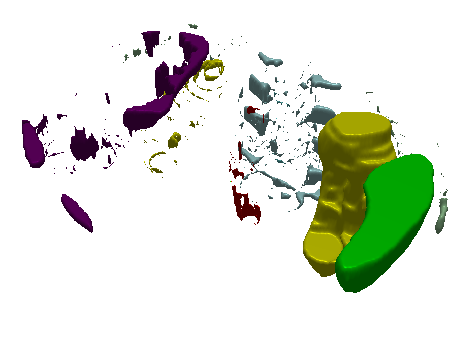
\includegraphics[width=.45\linewidth]{validation/validation-EB-2-60-80-GminusT.png}}%
\caption{A visual comparison of the automated and gold standard results for the EB-2-60-80 feature identification case study}
\label{fig:validation-EB-2-60-80}
\end{stusubfig}
%---

%---
\stufigex{height=8cm}{validation/validation-EB-2-60-80-leftkidney-tumour.png}{This slice shows why the automated identifier misses EB's left kidney -- we are trying to identify the region bounded by the yellow contour (the gold standard result), but the large tumour affecting the kidney causes the remaining kidney region to be too small to be identified successfully}{fig:validation-EB-2-60-80-leftkidney-tumour}{p}
%---

%---
\stufigex{height=8cm}{validation/validation-EB-2-60-80-spleen-missed.png}{The spleen is missed in the EB-2 case study because there is no suitable spleen seed in layer $1$ (all the regions are too small). The gold standard outline of the spleen is shown in green, for comparison purposes.}{fig:validation-EB-2-60-80-spleen-missed}{p}
%---

\index{validation!of 3D feature identifiers|)}

\afterpage{\clearpage}
\newpage

%##################################################################################################
\section{Validation of Volume Calculations}
%##################################################################################################

\index{validation!of volume calculations|(}

The ideal way to validate my volume calculations would have been to correlate them with real-world volumes calculated independently by the medics, but unfortunately these were not available. However, I was able to obtain the \emph{masses} of patients' organs calculated post-mortem as part of a study into the feasibility of performing virtual autopsies. These provided a reasonable (if not perfect) substitute for the volumes, since the major soft-tissue organs have known, and roughly uniform, densities (this is why they appear homogeneous on CT scans, since the Hounsfield scale used for CT images measures radiodensity). In conjunction with Dr Zoe Traill, the radiologist, it was therefore decided to focus on four different features -- the left and right kidneys, liver and spleen. I drew round these features in $19$ series ($740$ slices in total), with the results being checked, and corrected where necessary, by Dr Traill. The calculated volumes (in $\mathit{cm}^3$) resulting from this manual feature identification process are shown in Table~\ref{tbl:validation-volcalc}, alongside the corresponding masses (in $g$) calculated during the autopsies.

When drawing round the features, I was careful to include any cysts on the kidneys, as Dr Traill asserted that these would have been included when weighing the organs during the autopsy. In one case -- for the right kidney of patient OX46 -- this significantly affected the result, due to a large ($80\mathit{mm}$ diameter) cyst being included in the volume calculation whilst not appearing to affect the mass in a similar way. It was hypothesised that this may have been due to the cyst bursting before the kidney was weighed. For that reason, the result in question was specifically excluded as an outlier.

As shown in Table~$3$ of \cite{woodard86}, the accepted densities of the kidneys, liver and spleen are respectively $1050 \; \mathit{kg} \; m^{-3} = 1.05 \; g \; \mathit{cm}^{-3}$, $1050$--$1070 \; \mathit{kg} \; m^{-3} = 1.05$--$1.07 \; g \; \mathit{cm}^{-3}$ and $1060 \; \mathit{kg} m^{-3} = 1.06 \; g \; \mathit{cm}^{-3}$. The validation method involved graphing volumes (on the $x$ axis) against masses (on the $y$ axis) for each feature. Given the uniform densities of the organs involved, each graph was expected to be linear. It was therefore possible to fit a linear regression line in each case, whose gradient was expected to be reasonably close to the accepted density of the feature in $g \; \mathit{cm}^{-3}$.

As illustrated by the graphs in Figures~\ref{fig:validation-volcalc-leftkidney} to \ref{fig:validation-volcalc-spleen}, these expectations were largely borne out. To $2$ decimal places, the densities (in $g \; \mathit{cm}^{-3}$) of the organs as calculated from the linear regression lines on the graphs were $1.15$ for the left kidney, $1.12$ for the right kidney, $1.07$ for the liver and $1.14$ for the spleen. These were considered to be reasonably good results, especially for the liver.

There are number of sources of potential inaccuracy which can explain the discrepancies between the calculated densities and the accepted densities provided in \cite{woodard86}:
%
\begin{enumerate}

\item At the volume calculation end, it is sometimes very difficult even for an experienced radiologist to be certain of the precise boundary round a given organ -- indeed, subjectivity between different radiologists is a well-known issue in medical imaging (e.g.~see \cite{sampat06}). Since the series used for validation here were all imaged post-mortem (and thus without the benefit of a contrast agent), being certain of the precise boundaries was more than usually difficult for some patients in this case.

\item At the mass calculation end, the precise masses calculated depend on the way in which the organs are resected during the autopsies. It is highly unlikely that anyone performing an organ resection would be able to attain an organ boundary that precisely matched that shown on the CT scan.

%(Indeed, having witnessed an operation in the past and seen some of the difficulties involved in surgical procedures, I find it encouraging that the results match up as closely as they do in this case.)

\item In many of the series being validated, cysts were present on one or both kidneys. Depending on the type of cyst involved, these were either more or less dense than the adjoining kidney tissue, thus affecting the uniform density assumption. In most cases, however, these cysts were not large enough to significantly affect the results.

\end{enumerate}
%
Given the above factors affecting the results, I consider that my volume calculation method itself is relatively accurate. From a medical perspective, this suggests that it may be possible to predict the masses of organs by using volumes calculated from CT scans. This could be useful in cases where it is considered undesirable to perform an autopsy.

%---
\begin{landscape}
\begin{table}[p]
\footnotesize
\begin{center}
\begin{tabular}{c|rrc|rrc|rr|rr}
\textbf{Patient} & \multicolumn{3}{|c|}{\textbf{Left Kidney}} & \multicolumn{3}{|c|}{\textbf{Right Kidney}} & \multicolumn{2}{|c|}{\textbf{Liver}} & \multicolumn{2}{|c}{\textbf{Spleen}} \\
& \emph{Mass} ($g$) & \emph{Vol.} ($\mathit{cm}^3$) & \emph{Cysts} $> 5\mathit{mm}$ & \emph{Mass} ($g$) & \emph{Vol.} ($\mathit{cm}^3$) & \emph{Cysts} $> 5\mathit{mm}$ & \emph{Mass} ($g$) & \emph{Vol.} ($\mathit{cm}^3$) & \emph{Mass} ($g$) & \emph{Vol.} ($\mathit{cm}^3$) \\
\hline
\hline
OX25 & 120 &  96.116 &            --- & 110 &  96.044 &                            --- & 1680 & 1468.657 & 110 & 105.568 \\
OX26 & 190 & 173.155 &            --- & 190 & 175.411 &                            --- & 1790 & 1752.384 &  40 &  32.879 \\
OX27 &  80 &  74.897 &              6 &  85 &  84.300 &                             12 & 1370 & 1156.192 & 140 & 121.837 \\
OX29 & 110 & 106.566 &            --- &  90 &  94.306 &                            --- & 1380 & 1323.991 & 170 & 121.665 \\
OX30 & 120 & 126.524 &         28, 27 & 120 & 113.079 &                              9 & 1819 & 1662.805 & 180 & 158.506 \\
OX31 & 200 & 175.163 &             14 & 170 & 153.155 &                            --- & 2120 & 1972.002 & 110 &  98.132 \\
OX33 & 120 & 111.776 &         12, 10 & 110 & 105.223 &                             10 & 1010 & 1042.976 & 110 &  98.362 \\
OX34 & 100 &  91.514 &            --- & 110 &  93.505 &                            --- &  880 &  792.150 &  70 &  65.271 \\
OX35 &  95 &  93.405 &             32 &  90 &  81.308 &                            --- & 1120 & 1091.544 &  45 &  35.542 \\
OX36 & 170 & 147.269 & 25, 19, 17, 10 & 140 & 126.720 & 15 ($\times$4), 10 ($\times$2) & 1660 & 1410.233 & 260 & 237.772 \\
OX37 & 160 & 132.421 &             23 & 140 & 110.786 &                            --- & 1210 & 1016.613 & 120 &  91.921 \\
OX38 & 126 & 114.638 & 24, 18, 13, 12 & 134 & 112.267 &                            --- & 1387 & 1501.876 & 196 & 203.940 \\
OX39 & 125 & 105.321 &            --- & 120 & 113.161 &                            --- & 1250 & 1212.430 & 120 & 104.221 \\
OX40 & 140 & 121.521 &            --- & 140 & 117.883 &                            --- & 1390 & 1297.704 & 110 &  78.971 \\
OX41 & 150 & 110.221 &            --- & 120 &  94.978 &                            --- & 1670 & 1577.043 & 150 & 124.464 \\
OX42 & 230 & 183.583 &            --- & 180 & 160.707 &                            --- & 1650 & 1565.364 & 100 &  85.891 \\
OX43 & 140 & 111.631 &            --- & 150 & 124.826 &                            --- & 1200 & 1066.671 & 190 & 165.091 \\
OX44 & 140 & 111.968 &            --- & 130 & 112.832 &                            --- & 1440 & 1344.238 & 130 &  83.531 \\
OX46 & 130 & 115.295 &            --- & 130 & 303.460 &                             80 & 1000 & 1020.945 &  90 &  81.773
\end{tabular}
\end{center}
\caption{Tabulating my organ volume calculations for the kidneys, liver and spleen with organ masses calculated during the autopsies of $19$ patients. The series used were from a study into the feasibility of performing virtual autopsies. Patients OX28, OX32 and OX45 were excluded, due to their data not being available at the time of validation.}
\label{tbl:validation-volcalc}
\end{table}
\end{landscape}
%---

%---
\stufigex{height=9cm}{validation/validation-volcalc-leftkidney.png}{Graphing my left kidney volume calculations against the left kidney masses calculated during the autopsies}{fig:validation-volcalc-leftkidney}{p}
%---

%---
\stufigex{height=9cm}{validation/validation-volcalc-rightkidney.png}{Graphing my right kidney volume calculations against the right kidney masses calculated during the autopsies}{fig:validation-volcalc-rightkidney}{p}
%---

%---
\stufigex{height=9cm}{validation/validation-volcalc-liver.png}{Graphing my liver volume calculations against the liver masses calculated during the autopsies}{fig:validation-volcalc-liver}{p}
%---

%---
\stufigex{height=9cm}{validation/validation-volcalc-spleen.png}{Graphing my spleen volume calculations against the spleen masses calculated during the autopsies}{fig:validation-volcalc-spleen}{p}
%---

\index{validation!of volume calculations|)}

\clearpage
\newpage

%##################################################################################################
\section{Chapter Summary}
%##################################################################################################

In this chapter, both my feature identification work and volume calculation method were validated against `gold standard' results produced in collaboration with a radiologist. The next chapter critically assesses both the feature identification work validated here and the other original contributions claimed in Chapter~\ref{chap:introduction}.
